\documentclass[conference]{IEEEtran}
\IEEEoverridecommandlockouts
% The preceding line is only needed to identify funding in the first footnote. If that is unneeded, please comment it out.
\usepackage{cite}
\usepackage{amsmath,amssymb,amsfonts}
\usepackage{algorithmic}
\usepackage{graphicx}
\usepackage{textcomp}
\usepackage{cite}
\usepackage{algorithmic}
\usepackage{graphicx}
\usepackage{textcomp}
\usepackage[dvipsnames]{xcolor}
\usepackage{paralist}
\usepackage[inline]{enumitem}
\usepackage{caption}
\usepackage{multirow}
\usepackage{booktabs}
\usepackage{makecell}
\usepackage{tabu, booktabs}
\usepackage{float}
\usepackage{subcaption}
\usepackage{pifont}
\usepackage{comment}
\usepackage{todonotes}
\usepackage{hyperref}
\usepackage{csquotes}
\usepackage{multirow}
\usepackage{booktabs}
\usepackage{graphicx}
\usepackage{epstopdf}
\usepackage{color}
\usepackage{gnuplottex}
\usepackage{graphicx}
\usepackage{epstopdf}
\usepackage{pgf}


\newcommand\myshade{85}

\pdfobjcompresslevel=0
\pdfminorversion=4


\definecolor{magma_darker}{HTML}{fdc38a}
\definecolor{magma_dark}{HTML}{e15666}
% \definecolor{magma_light}{HTML}{82s247f}
\definecolor{magma_lighter}{HTML}{1f0c43}

\definecolor{cvpr_link}{HTML}{00ffff}
\definecolor{cvpr_cite}{HTML}{00ff00}
\definecolor{cvpr_file}{HTML}{ff0000}

\definecolor{royalblue}{RGB}{65, 105, 225}
\definecolor{darkgreen}{RGB}{0, 100, 0}
\definecolor{darkred}{RGB}{139, 0, 0}
\definecolor{darkviolet}{RGB}{148, 0, 211}

\colorlet{linkColor}{violet}
\colorlet{citeColor}{YellowOrange}
\colorlet{urlColor}{Emerald}

\hypersetup{
  linkcolor  = darkviolet!\myshade!black,
  citecolor  = citeColor!\myshade!black,
  urlcolor   = urlColor!\myshade!black,
  filecolor  = darkgreen!\myshade!black,
  colorlinks = true,
}
\usepackage[a4paper, total={184mm,239mm}]{geometry}
\def\BibTeX{{\rm B\kern-.05em{\sc i\kern-.025em b}\kern-.08em
    T\kern-.1667em\lower.7ex\hbox{E}\kern-.125emX}}

\ExplSyntaxOn
\DeclareExpandableDocumentCommand{\convertlen}{ O{cm} m }
 {
  \dim_to_decimal_in_unit:nn { #2 } { 1 #1 } cm
 }
\ExplSyntaxOff
\usepackage{gnuplottex}
\usepackage{tikz}
\usepackage{mathtools}
\newcommand{\ra}[1]{\renewcommand{\arraystretch}{#1}}
\usetikzlibrary{matrix,calc,positioning,arrows.meta}

\newcommand{\omark}{\ding{51}}
\newcommand{\cmark}{\ding{52}}

\DeclarePairedDelimiter\ceil{\lceil}{\rceil}
\DeclarePairedDelimiter\floor{\lfloor}{\rfloor}

\DeclareMathOperator*{\argmax}{arg\,max}
\DeclareMathOperator*{\argmin}{arg\,min}

\newcommand{\abs}[1]{\lvert#1\rvert}
\newcommand{\Abs}[1]{\left\lvert#1\right\rvert}

\newcommand{\deriv}[2][x]{\frac{\mathrm{d}#2}{\mathrm{d}#1}}
\newcommand{\adj}[1]{\mathrm{adj}(#1)}
\newcommand{\spec}[1]{\mathrm{spec}(#1)}
\newcommand{\diag}[1]{\mathrm{diag}(#1)}
\newcommand{\tril}[1]{\mathrm{tril}(#1)}
\newcommand{\triu}[1]{\mathrm{triu}(#1)}
\newcommand{\chol}[1]{\mathrm{chol}(#1)}
\newcommand{\sinc}[1]{\mathrm{sinc}\left(#1\right)}

\newcommand{\stimes}{{\times}}

\newcommand*\circled[1]{\tikz[baseline=(char.base)]{\node[shape=circle,fill,inner sep=0.5pt] (char) {\textcolor{white}{#1}};}}
\newcommand*\pilar[3]{\tikz[baseline=(char.base)]{\node[shape=circle,fill=#2,inner sep=0.5pt] (char) {\textcolor{#3}{#1}};}}

\newcommand\norm[1]{\left\lVert#1\right\rVert}

\newcommand{\red}[1]{{\color{red}#1}}
\newcommand{\blue}[1]{{\color{blue}#1}}

% If your conference documentclass or package defines these macros,
% change these macros to different names.
\newcommand*{\affaddr}[1]{#1} % No op here. Customize it for different styles.
\newcommand*{\affmark}[1][*]{\textsuperscript{#1}}
\newcommand*{\email}[1]{#1}
\setlength {\marginparwidth }{2cm}
\begin{document}

\title{Late Breaking Results: Leveraging Approximate Computing for Carbon-Aware DNN Accelerators}

\author{
\IEEEauthorblockN{
Aikaterini Maria Panteleaki\IEEEauthorrefmark{1},
Konstantinos Balaskas\IEEEauthorrefmark{2},
Georgios Zervakis\IEEEauthorrefmark{2},
Hussam Amrouch\IEEEauthorrefmark{3},
Iraklis Anagnostopoulos\IEEEauthorrefmark{1}
}
\IEEEauthorblockA{
\IEEEauthorrefmark{1}Southern Illinois University Carbondale, 
\IEEEauthorrefmark{2}University of Patras, 
\IEEEauthorrefmark{3}Technical University of Munich
}
}

\maketitle
\begin{abstract}
Retrieval-Augmented Generation (RAG) is often used with Large Language Models (LLMs) to infuse domain knowledge or user-specific information. In RAG, given a user query, a retriever extracts chunks of relevant text from a knowledge base. These chunks are sent to an LLM as part of the input prompt. Typically, any given chunk is repeatedly retrieved across user questions. However, currently, for every question, attention-layers in LLMs fully compute the key values (KVs) repeatedly for the input chunks, as state-of-the-art methods cannot reuse KV-caches when chunks appear at arbitrary locations with arbitrary contexts. Naive reuse leads to output quality degradation.  This leads to potentially redundant computations on expensive GPUs and increases latency. In this work, we propose \sys, a system for managing and reusing precomputed KVs corresponding to the text chunks (we call \textit{chunk-caches}) in RAG-based systems. We present how to identify \hl{\textit{chunk-caches} that are reusable}, how to efficiently perform a small fraction of recomputation to \textit{fix} the cache to maintain output quality, and how to efficiently store and evict \textit{chunk-caches} in the hardware for maximizing reuse while masking any overheads. With real production workloads as well as synthetic datasets, we show that \sys reduces redundant computation by \textbf{51\%} over SOTA prefix-caching and \textbf{75\%} over full recomputation.
\hl{Additionally, with continuous batching on a real production workload, we get a \textbf{1.6$\times$} speedup in throughput and a \textbf{2$\times$} reduction in end-to-end response latency over prefix-caching while maintaining quality, for both the \llama-3-8B and \llama-3-70B models. 
}
\end{abstract}






\begin{IEEEkeywords}
Approximate Accelerators, Embodied Carbon Footprint, Sustainable Computing
\end{IEEEkeywords}

\documentclass[../main.tex]{subfiles}
\graphicspath{{../images/}}
\makeatletter
\def\input@path{{../images/}}
\makeatother
\begin{document}
\section{Introduction}
\begin{figure}
\centering
\begin{tikzpicture}
\node[inner sep=0pt] (ws) at (0, 0) {
\includegraphics[height=.4\textwidth, trim={10cm 0 10cm 0},clip]{world_space.png}};
\node[inner sep=0pt] (cs) at (6,0) {\includegraphics[height=.4\textwidth, trim={10cm 1cm 10cm 4cm},clip]{conf_space.png}};
\end{tikzpicture}
\vspace{-5pt}
\label{fig:pbrm_intro}
\caption{\textbf{Left}: Shows world space obstacles as grey spheres. Robots start and goal configuration is colored red and green, respectively. Configurations along the computed path are colored transparent blue. \textbf{Right:} Mapped world space scenario to configuration space. Obstacle region is the grey mesh. Red spheres are collision-free regions computed by the neural SCDF. The optimized shortest path in the convex corridor is the blue curve.}
\vspace{-25pt}
\end{figure}
Motion planning is the problem of finding a collision-free trajectory that connects a given start and goal configuration. The planning takes place in the configuration space of the robot. For single body robots, like mobile robots or drones, the configuration space and the world space are usually the same. This simplifies the planning, since explicit obstacle representations are available which enables geometrical tools like separating hyperplanes, smallest distance to obstacles etc., to be used when designing motion planning algorithms. For multi-body robots like manipulators, the situation is completely different. The world space obstacles are usually mapped to non-convex regions, and to make the problem even harder, the mapping is usually not known. Forming explicit representations of the obstacle region in the configuration space is usually too expensive or intractable. Despite all of this, sampling based planners are used with great success, which mainly is due to their use of implicit representations of the obstacle region. The basic idea is to construct a graph in the configuration space that covers and connects the collision-free region. From this graph, a path can be extracted that connects a given start and goal configuration. The approach is computationally expensive, since the graph is constructed with the smallest geometrical building block available, points, which represents a collision-check. Furthermore, the extracted paths from the graph are non-smooth and jagged due to the stochastic nature of the approach. This adds an additional post-processing step to the process, where the paths are shortcutted and smoothened, before the path can be used for tracking. Clearly a lot of time is invested to form this graph and produce smooth paths. Thus, if the obstacles start to move, then all of this work is done in no use, since all points that make up this graph need to be re-verified, which is simply too time consuming to be done in real time.
\\\\
In this work, we want to address the existing drawbacks of the sampling based planners. Our main contribution is an improved motion planner where each vertex in the graph covers a collision-free region in the form of a sphere instead of a point and where the edges are formed with neighboring intersecting spheres. This representation has the advantage of instead of returning piecewise linear paths, returning a sequence of overlapping spheres, i.e. a convex corridor, that connects a given start and goal configuration, illustrated in Figure \ref{fig:pbrm_intro}. This convex corridor allows us to use convex optimization to produce smooth trajectories, instead of computationally expensive post-processing methods. The representation further allows us to estimate the coverage of the collision-free space, which gives us awareness and feedback in the offline roadmap construction phase. Finally, our representation is simple to adapt to moving obstacles, simply requery for the new radii and recheck for intersections. 
\\\\
The spherical collision-free regions are formed using a signed distance function (SDF), which is a function that returns the smallest distance from an arbitrary point to the boundary of an obstacle. As the name implies, the distance is signed, thus if the point is inside the obstacle it is negative otherwise positive. If the distance is positive, a sphere with radius equal to the distance is guaranteed to cover a collision-free region. Using an SDF in motion planning is not new, but what is novel about our approach is that we express the distance in the configuration space instead of the world space and by doing so allows us to form these convex collision-free regions. We refer to the resulting SDF as a signed configuration distance function (SCDF). Computing an SCDF analytically is non-trivial, our approach is therefore to parameterize the SCDF with a deep neural network and learn the mapping by supervised learning. Our resulting neural SCDF can compute distances for different parameter values of obstacle shapes and we also show how multiple distances can be combined, thus making our approach flexible.
\section{Related work}
Motion planning algorithms can roughly be divided into three families, grid-based, sampling based and optimization based methods. Grid-based methods (GBM) discretize the planning space from which a graph is then compiled. A standard search method is A$^\star$ \citep{a_star}, which is classified as an \textit{informed} search method, since it employs a heuristic function to speed up the search. A$^\star$ guarantees to return an optimal path at the level of discretization used. GBMs usually discretize the planning space by a regular lattice and this limits the GBMs to problems with low dimensionality due to the curse of dimensionality. Thus, GBMs are usually limited to single-body robots where the degrees of freedom (DOF) are low. To overcome the inherent scaling problem with the GBMs, stochastic methods are usually used for multi-body robots. These methods are termed as sampling-based methods (SBM) and core members within this family are the rapidly-exploring random trees (RRT) \citep{rrt} and the probabilistic roadmap (PRM) \citep{prm}. RRT grows a tree from the start configuration and explores the collision-free region in a rapid way until it is able to connect to the goal region. RRT is usually improved by bi-directional planning \citep{rrt_connect}, i.e. an additional tree is grown from the goal configuration and the trees are tested for connection after any tree has been expanded. RRT is a single-query method, thus it searches for a path from scratch each time it is queried. Contrary to this, PRM is a multi-query method, which solves for multiple queries without starting from scratch. PRM does this by creating a roadmap (graph) that covers the collision-free space as an offline step. The graph is then used to solve for multiple queries. PRMs are used in cases where the environment does not change since the extra offline step is too computationally costly and needs to be re-done if the environment is changed. In our work, we address this inherent issue by using a different roadmap representation. Our vertices in the graph cover a collision-free region in the form of spheres and we form the edges by checking for intersecting spheres. If something in the environment changes, we recompute the spheres radii and recheck the intersections, without relying on collision detection. We use a trained neural network to compute the sphere radius, therefore querying for the radius can be done fast, hence our representation enables the PRM for dynamic environments.
\\\\
In the recent decades, optimization based methods (OBM) \citep{chomp, schulman, itomp, stomp} have been introduced as an alternative to SBM for multi-body robots. Like the SBM, the OBMs scale well to higher dimensional problems and produce smoother motion. It is common to use a SDF in the optimization since it is a smooth function, thus enabling gradient-based methods. However, the standard way of expressing the SDF is in world space. The distance therefore needs to be mapped to the configuration space by the forward kinematics. This mapping makes the optimization problem a non-linear program (NLP), which is computationally expensive to solve. Recently, a different approach has been proposed. In \cite{mp_gcs} motion planning is formulated as a convex optimization problem by using the graph of convex sets framework \citep{gcs}. The underlying idea is to decompose the collision-free space into intersecting convex sets from which a convex optimization problem is formulated. In cases where an explicit representation of the obstacles in the configuration space exists, like for single-body robots, creating collision-free convex regions can be done fast \citep{iris}. For multi-body robots, this is non-trivial. Existing work does this successfully \citep{iris_nlp, iris_c} by an optimization based approach, but the methods are still too time consuming to be used in the presence of moving obstacles. Our approach is instead to use deep learning to learn an SDF expressed in the configuration space. With this, we can query for shortest distances to the collision boundary, which allows us to expand spherical regions which are collision-free. Our approach is fast and therefore enables our suggested roadmap planner to be used in dynamic environments.
\\\\
Recent research has focused on learning collision detection \citep{fk_kernel_distance, diffco, graphdistnet} by predicting the signed distance between the robot links and the surrounding obstacles in the world space. The learned SDF is used in trajectory optimization but since the distance is expressed in the world space, the problem becomes an NLP and therefore takes a long time to solve. We take a novel approach and suggest to instead express the signed distance in the configuration space. This allows us to improve the PRM at the same time as it enables convex optimization for trajectory optimization, which runs faster and is more reliable than NLP solvers. In \cite{cspf} a learned signed distance function in the configuration space is proposed similar to our approach. However, their approach is restricted to point cloud representations, while we propose to represent the obstacles as parameterized geometric shapes, e.g. spheres. Furthermore, we also show how to use our learned SCDF to improve an existing roadmap planner.
\section{Problem formulation}
A robot is located in the world space, $\W \subset \R^3 $. The unique location of the robot is given by its configuration $\q \in \C$, where $\C$ is the configuration space. The set of points covered by the robots bodies at a certain configuration is expressed as $\B(\q) \subset \W$. The robot is surrounded by $\NrObst$ obstacles $\O = \bigcup_{i=1}^{\NrObst} \O_i$, where  $\O_i \subset \W$. The representation of the obstacle in the configuration space is the set $\C\O_i = \{\q \in \C \: |\: \B(\q) \cap \O_i \neq \emptyset \}$. The obstacle space is formed as $\Co = \bigcup_{i=1}^{\NrObst} \C \O_i$. The complement is referred to as the free space, $\Cf = \C \setminus \Co$. The path planning problem is a tuple, ($\Cf$, $\qStart$, $\qGoal$), where we want to connect a query pair, consisting of a start, $\qStart$, and goal configuration, $\qGoal$, with a geometric path, $\q(s): [0, 1] \mapsto \Cf$, such that $\q(0)=\qStart$ and $\q(1)=\qGoal$, or report correctly when such a path does not exist.
\end{document}


\section{\label{sec:method}Methodology}

Each SIEM system uses its own RDL to define threat detection rules, and each RDL has its own schema.
For example, the Splunk SIEM uses the SPL to define its threat detection rules.
The task of understanding threat detection rules and recommending relevant MITRE ATT\&CK techniques (or sub-techniques) requires complex reasoning skills.
In the case of LLMs, this can be achieved with a technique called prompt chaining in which each task is divided into multiple sub-tasks in order to understand the complex reasoning behind the task.
Therefore, we employ a multi-phase architecture based on prompt chaining that leverages the power of LLMs to take a SIEM rule defined in any RDL and map it to relevant MITRE ATT\&CK techniques using the power of LLMs.
Our approach is based on the following intuitions:
\begin{itemize}[nosep,leftmargin=*]
    \item \textit{LLMs' implicit knowledge}: LLMs possess deep understanding of diverse RDLs. This enables them to interpret any rule, regardless of the RDL it is defined in, and convert it into comprehensible natural language text.
    \item \textit{LLMs' similarity comparison capability}: LLMs are adept at analyzing and comparing textual descriptions. 
    They can intelligently assess the similarity between two textual inputs to establish a meaningful connection.
\end{itemize}

\methodName has two main phases: (1) the rule to text translation phase, and (2) the MITRE ATT\&CK techniques recommendation phase.
These two phases in the pipeline include six key steps to determine relevant TTPs, as illustrated in Figure~\ref{fig:r2t}.

Although LLMs excel at translating SIEM rules into natural language, they often lack critical domain-specific contextual information related to IoCs in the rules.
To overcome this limitation, the \textit{rule to text translation} phase includes three steps: IoC extraction, contextual information retrieval, and natural language translation.

The workflow begins with the extraction of IoCs from the rules (for example, processes, log source, event codes, and file names) that the rule searches for in the logs (step (1)).In the next sstep a web search agent performs the task of obtaining additional contextual information about the IoCs discovered ((step 2)).
By incorporating this additional domain-specific information, the pipeline enhances the language translation, resulting in a more accurate and meaningful interpretation of SIEM rules.
The rule itself and the IoCs' contextual additional information from the previous stage are then used to translate the rule from RDL to natural language (step (3)).

The \textit{MITRE ATT\&CK techniques} recommendation phase of the pipeline includes the following three steps.
The rule in processed in data source identification step in which the probable origin of the data is identified (step (4)).
The description of the rule is then used to determine probable MITRE ATT\&CK techniques based on the implicit knowledge of the LLM (step (5)).
Finally, using chain-of-thought~\cite{wei2022chain} prompting, the most relevant techniques are extracted from the list of probable techniques (step (6)).
Each step of our method is further described in detail below.


% [bb=0 0 1440 900,width=1.43\linewidth,height=0.9\textwidth]
\begin{figure*}[htbp]
   \includegraphics[width=\textwidth]{Images/stages.jpg}
    
   \caption{An illustration of the different steps in \methodName.}
   \label{fig:stages}
\end{figure*} 

\subsection{IoC Extraction}
The context associated with a SIEM detection rule is crucial for its accurate interpretation and effective application. 
Obtaining this contextual understanding requires comprehensive analysis of the embedded IoCs in the SIEM rule.
In the first step, \methodName systematically identifies and extracts all IoCs, identifying the types of IoCs and their corresponding values that form the foundational elements of the detection rules. 
Leveraging the LLM's inherent understanding of rule structures and IoCs, we employ a zero-shot prompting approach for this task. 
Zero-shot prompting enables the direct extraction of IoCs from the rules without requiring extensive pre-training on specific datasets.

\noindent The result of this stage is a dictionary structure, where:
\begin{itemize}[nosep,leftmargin=*]
    \item Keys represent types of IoC, such as processes, files, IP addresses, and log sources.
    \item Values are lists containing specific IoC details, such as process names, file names, IP addresses, and log source identifiers.
\end{itemize}

In the example depicted in Figure~\ref{fig:stages}(a), the pipeline processes a rule for which relevant MITRE ATT\&CK techniques need to be recommended. 
The IoC extractor LLM produces a dictionary structure as output, organizing the IoCs in a structured format to support subsequent stages in the analysis pipeline. 



\subsection{Contextual Information Retrieval}
In this step, an LLM agent is employed to retrieve relevant information pertaining to the IoCs extracted from the rule.
A REACT agent~\cite{react} was used in this case to generate both reasoning traces and task-specific actions in an interleaved manner.
REACT agents interact with external tools to retrieve additional information that leads to more factual and reliable responses.
The LLM agent conducts a systematic search across web resources to gather additional contextual information for each IoC value present in the rule. 
This step addresses LLMS' lack of up-to-date knowledge or specialized domain expertise (which is critical to understanding the role and significance of the IoCs in the rule), without the need for retraining or fine-tuning.
Figure~\ref{fig:stages}(b) presents an example in which the rule includes the process name \texttt{soaphound.exe} as an IoC.
As can be seen, the web search results indicate that \texttt{soaphound.exe} is being used for active directory (AD) enumeration, which is important for the understanding of the attack. 

\subsection{Natural Language Translation}

The translation of detection rules into natural language textual descriptions fulfills three key objectives:
\begin{enumerate}[nosep,leftmargin=*]
    \item \textbf{Ensures that \methodName is format-agnostic}: It converts rules defined in various RDL formats into a generic, unstructured text format, ensuring compatibility with different SIEM systems, regardless of the specific rule format.
    \item \textbf{Provides contextual explanation}: It includes all relevant contextual information to produce a concise and comprehensible explanation of the rule.
    \item \textbf{Enhances the comprehension for LLMs}: It enables LLMs to more effectively compare the translated rule with descriptions in the MITRE ATT\&CK framework by providing a unified textual representation.
\end{enumerate}
To achieve these objectives, a zero-shot prompting technique is employed. 
The input to the LLM comprises two components:
\begin{itemize}
    \item \textbf{Syntactical information}: The rule itself, providing the structural and operational details.
    \item \textbf{Contextual information}: Details of the IoCs extracted from the rule, providing semantic insights into the rule's intent and function.
\end{itemize}
The LLM utilizes these inputs to generate a natural language textual description of the rule. 
This transformation not only ensures a more interpretable representation but also facilitates further steps of analysis and comparison, particularly in aligning the rule with MITRE ATT\&CK techniques and sub-techniques.



\subsection{Data Source or Mitigation Identification}
Identifying the most relevant data component or mitigation associated with the rule description in this step is critical for filtering out irrelevant MITRE ATT\&CK techniques (or sub-techniques) in subsequent steps of the pipeline.
In the MITRE ATT\&CK framework, data sources represent various categories of information that can be gathered from sensors or logs. 
These data sources include \textit{data components}, which are specific attributes or properties within a data source that are directly relevant to detecting a particular technique or sub-technique~. 
For example, in the context of the rule described in Figure~\ref{fig:stages}(a), the term \texttt{Endpoint.Processes} indicates that the activity is happening on an endpoint. 
Presence of the terms such as, \texttt{soaphound.exe}, \texttt{--buildcache}, \texttt{--certdump} and etc. indicate that the rule searches for command line execution of an executable named \texttt{soaphound.exe} with specific parameters. 
Therefore, the appropriate data source in this example is \textit{Command}, with the corresponding data component being \textit{Command Execution}.
Additionally, \textit{mitigations} are defined as categories of technologies or strategies that can prevent or reduce the impact of specific techniques or sub-techniques. 
The MITRE ATT\&CK framework explicitly establishes relationships between data components, mitigations, and techniques (or sub-techniques), enabling a systematic approach for identifying relevant elements.

To identify the most relevant data component or mitigation associated with a given rule description, we utilize agentic retrieval augmented generation (RAG), which incorporates an AI Agent-based implementation of the RAG framework.
Data from the MITRE ATT\&CK framework, specifically related to data components and mitigations, is stored in a vector database (e.g., ChromaDB). 
The process begins with the rule description from the previous stage, which serves as the input to the AI Agent. 
The LLM-powered agent automatically generates a search query tailored to retrieve relevant information from the RAG database.

For each query, the system retrieves the five most similar documents from the database, each containing contextual information about data components or mitigations. 
These documents are then utilized by the LLM agent to contextualize the rule description. 
By comparing the content of these retrieved documents with the rule description, the LLM agent determines and outputs the most relevant data component or mitigation along with a chain-of-thought as to why the data component or mitigation is related to the rule.


\subsection{Probable Technique Recommendation}

In this step, an LM agent is utilized to propose probable MITRE ATT\&CK techniques (and sub-techniques) that may be relevant to the description of the provided rule.
We used a REACT agent in this step as well to utilize both implicit and explicit knowledge during reasoning.
For explicit knowledge, the agent searches the MITRE ATT\&CK framework to obtain the list of probable techniques (and sub-techniques).
The natural language description of the rule from the previous step serves as input to the LLM agent.
The output of this stage consists of a list of JSON objects, each containing the MITRE technique ID, technique name, and technique description as seen in Figure~\ref{fig:stages}(c).

Throughout our experiments, we observed that as the number of recommendations ($k$) increases, both the framework's average recall and precision initially improve, however beyond a certain threshold of $k$, the %average 
precision begins to decline.
Based on these observations(please refer Table~\ref{tab:results3}), we selected a $k$-value of 11 to ensure a high recall.



\subsection{Relevant Technique Extraction}
In this step, \methodName refines the set of probable MITRE ATT\&CK techniques identified in the previous stage by eliminating irrelevant entries.
This step in the pipeline serves two primary purposes: (1) to enhance precision while maintaining recall achieved in previous step, and (2) to provide a clear rationale for the selection of the labels, ensuring transparency and interpretability of the mapping process.
This refinement process is grounded in the assumption that LLMs are effective for text similarity matching tasks.

The process comprises two key steps:
\begin{itemize}
    \item \textit{Rule-technique comparison}: The description of each technique in the set of probable techniques is compared with the rule description. 
    A chain-of-thought technique is then applied to elucidate the reasoning behind the association of each technique with the rule.
    \item \textit{Confidence calculation}: The generated chain-of-thought rationale for each technique (or sub-technique) is compared with the rule description to compute a relevance (or confidence) score, as done in prior work~\cite{freitas2024ai}.
    % \item \textbf{Reasoning}: \new{Add here the reasoning that it provides - explaining in NLP why it was selected...}
\end{itemize}

Techniques with higher confidence scores are deemed more relevant to the rule. 
Conversely, techniques with scores falling below a predefined threshold are excluded.
The techniques retained after this filtering step represent the most relevant techniques corresponding to the given rule's description. 


The chain-of-thought (CoT) rationale generated during the comparison of each rule to its probable technique is also provided as an output in this step.
This rationale offers a detailed natural language explanation, articulating why a particular technique is relevant to the given rule. 
Such explanations are highly valuable for security analysts, as they provide clear and transparent reasoning behind the mapping, enabling analysts to better understand and validate the association between the rule and the technique.
Other classification models proposed in previous works within this domain also suffer from the limitation of being black-box models, which lack the ability to provide clear reasoning or explanations. 
Unlike \methodName, these models fail to generate transparent, CoT rationales that explain why a particular rule is mapped to a specific technique, making them less interpretable and less useful for security analysts.
\section{Evaluation}
We provide three sets of insights into this section, organised as \textit{findings (F*)}. We quantitatively study the effect of the adversarial and counterfactual perturbations on the performance of informal reasoners and autoformalisation methods. Then, we dive deeper into method variants. Finally, 
we analyse the nature of formalisation errors made by the models.

\subsection{Robustness Analysis}
\paragraph{\textbf{\emph{F1: Noise perturbations have a stronger effect on formalisation methods than informal \ac{LLM} reasoners.}}}
Table~\ref{tab:distraction_k4_formalisation} shows that, on average, the accuracy of both direct and \ac{CoT} informal reasoning remains between $73\%$ and $74\%$ in the face of added noise. While the autoformalisation method performs similarly to informal reasoners on the original dataset, its performance decreases between $4\%$ and $11\%$. The accuracy drops especially with logical (L) and tautological (T) distractions, whose logical language formats trick the \ac{LLM} into formalizing the noisy clauses. On the other hand, the linguistically complex and more natural sentences of encyclopedic distractions show a minor effect, suggesting that \acp{LLM} successfully avoids formalizing the more complicated sentences.

\paragraph{\textbf{\emph{F2: All \ac{LLM}-based reasoning methods suffer a drop for counterfactual perturbations.}}} % influence .}}}
Table~\ref{tab:distraction_k4_formalisation} shows that counterfactual statements cause a significant decrease in performance for both the informal reasoners and autoformalisation methods of between $12\%$ and $13\%$ on average. 
Moreover, this observation also holds for all tested models, i.e., none are robust towards counterfactual perturbations across every evaluated dimension. Even the strongest model, GPT 4o-mini, yields a performance of 63-68\%, which is relatively close to the random performance of 50\%. The high impact of counterfactual statements (the single ``not'' inserted) could be due to the inability of \acp{LLM} to overwrite prior knowledge with explicitly stated information or memorization of the answers. We study the error sources further in §\ref{subsec:errors}.  

\noindent \paragraph{\textbf{\emph{F3: Introducing multiple noise sentences has an effect only for logical distractions.}}}
We show the impact of introducing between one and four sentences for the two top-performing autoformalisation models in Figure~\ref{fig:length_distraction}. The figure shows similar trends with and without counterfactual perturbations.
As additional logical distractions are introduced, the model performance consistently decreases. Tautological (T) distractions lead to a decline in accuracy with a single disruptive sentence, yet adding more noise does not worsen the outcome. 
The tautological corpus introduces truth constants for all sentences as a persistent unseen logical construct. Given that this leads only to a decrease for a single occurrence, we can assume that a model can consistently handle the same unseen logical construct. In contrast, the logical corpus increases the chance of adding text, requiring new, previously unseen reasoning constructs for each added sentence. The impact of encyclopedic noise remains negligible, generalising F1 to $k$ sentences. Similarly, counterfactual perturbations remain much more effective for all settings, generalising F2.

\begin{table}[!t]
\small
\setlength{\modelspacing}{2pt}
\setlength{\tabcolsep}{1.7pt} % Default value: 6pt
\setlength{\belowrulesep}{4pt}
\begin{threeparttable}
    \centering
    \begin{tabular}{cc l r rrr @{\quad} rrrr}
\toprule
\multirow{2}{*}{} & \multirow{2}{*}{} & Reasoning & \multirow{2}{*}{O} & \multicolumn{3}{c}{Distraction} & \multicolumn{4}{c}{Counterfactual} \\
 & & Format & & E& L & T & $\text{O}_C$ & $\text{E}_C$& $\text{L}_C$ & $\text{T}_C$\\
\midrule
\multirow{6}{*}{\rotatebox{90}{Gemma-2}} & \multirow{3}{*}{\rotatebox{90}{9b}}
   & Informal (direct) & \textbf{0.78} & \textbf{0.80} & \textbf{0.79} & \textbf{0.77} & 0.58 & 0.52 & 0.50 & 0.59 \\
 & & Informal (CoT) & 0.72 & 0.78 & 0.73 & 0.76 & 0.61 & \textbf{0.57} & \textbf{0.60} & \textbf{0.66} \\
 & & Formal (FOL) & 0.62 & 0.58 & 0.52 & 0.53 & \textbf{0.63} & 0.52 & 0.46 & 0.46 \\[\modelspacing]
\cmidrule{2-11}
 & \multirow{3}{*}{\rotatebox{90}{27b}} 
   & Informal (direct) & 0.71 & 0.69 & \textbf{0.66} & \textbf{0.68} & 0.59 & 0.51 & 0.54 & 0.59 \\
 & & Informal (CoT) & 0.66 & 0.65 & 0.64 & 0.63 & 0.62 & 0.58 & \textbf{0.62} & \textbf{0.64} \\
 & & Formal (FOL) & \textbf{0.74} & \textbf{0.74} & 0.61 & 0.61 & \underline{\textbf{0.72}} & \underline{\textbf{0.67}} & 0.58 & 0.51 \\[\modelspacing]
\midrule
\multirow{6}{*}{\rotatebox{90}{Mistral}} & \multirow{3}{*}{\rotatebox{90}{7B}} 
   & Informal (direct) & 0.77 & \textbf{0.77} & 0.75 & \textbf{0.79} & \textbf{0.63} & \textbf{0.54} & \textbf{0.54} & \textbf{0.66} \\
 & & Informal (CoT) & \textbf{0.79} & 0.75 & \textbf{0.77} & 0.78 & 0.55 & 0.52 & \textbf{0.54} & 0.58 \\
 & & Formal (FOL) & 0.62 & 0.58 & 0.54 & 0.57 & 0.50 & \textbf{0.54} & 0.51 & 0.52 \\[\modelspacing]
\cmidrule{2-11}
 & \multirow{3}{*}{\rotatebox{90}{Small}} 
   & Informal (direct) & \textbf{0.77} & \textbf{0.76} & \textbf{0.76} & \textbf{0.75} & 0.61 & 0.51 & 0.56 & 0.59 \\
 & & Informal (CoT) & 0.72 & 0.72 & 0.72 & 0.71 & \textbf{0.62} & \textbf{0.59} & \textbf{0.62} & \textbf{0.68} \\
 & & Formal (FOL) & 0.68 & 0.59 & 0.53 & 0.64 & 0.54 & 0.55 & 0.49 & 0.51 \\[\modelspacing]
\midrule
\multirow{6}{*}{\rotatebox{90}{Llama-3.1}} & \multirow{3}{*}{\rotatebox{90}{8B}} 
   & Informal (direct) & 0.63 & 0.61 & 0.64 & 0.66 & 0.61 & \textbf{0.62} & 0.59 & 0.61 \\
 & & Informal (CoT) & 0.73 & \textbf{0.73} & \textbf{0.71} & \textbf{0.72} & \textbf{0.62} & 0.59 & \textbf{0.61} & \textbf{0.65} \\
 & & Formal (FOL) & \textbf{0.77} & 0.71 & 0.63 & 0.52 & 0.60 & 0.58 & 0.55 & 0.52 \\[\modelspacing]
\cmidrule{2-11}
 & \multirow{3}{*}{\rotatebox{90}{70B}} 
   & Informal (direct) & 0.77 & 0.74 & 0.74 & 0.73 & 0.62 & 0.53 & 0.56 & 0.64 \\
 & & Informal (CoT) & \textbf{0.78} & \textbf{0.75} & \textbf{0.76} & \textbf{0.76} & 0.64 & 0.61 & \textbf{0.66} & \underline{\textbf{0.73}} \\
 & & Formal (FOL) & 0.74 & 0.73 & 0.71 & 0.71 & \textbf{0.66} & \textbf{0.62} & 0.59 & 0.57 \\[\modelspacing]
 \midrule
\multirow{3}{*}{\rotatebox{90}{GPT}} & \multirow{3}{*}{\rotatebox{90}{4o-mini}} 
   & Informal (direct) & 0.78 & 0.77 & 0.79 & 0.79 & 0.64 & 0.61 & 0.61 & 0.63 \\
 & & Informal (CoT) & 0.80 & 0.80 & \underline{\textbf{0.81}} & \underline{\textbf{0.82}} & \textbf{0.68} & \textbf{0.63} & \underline{\textbf{0.68}} & \textbf{0.64} \\
 & & Formal (FOL) & \underline{\textbf{0.84}} & \underline{\textbf{0.82}} & 0.73 & 0.79 & 0.63 & 0.62 & 0.57 & 0.54 \\[\modelspacing]
 \midrule
\multicolumn{2}{c}{\multirow{3}{*}{\textbf{Avg}}} 
 & Informal (direct) & 0.74 & 0.73 & 0.73 & 0.73 & 0.61 & 0.55 & 0.56 & 0.62 \\
 & & Informal (CoT) & 0.74 & 0.74 & 0.73 & 0.74 & 0.62 & 0.58 & 0.62 & 0.65 \\
  & & Formal (FOL) & 0.72 & 0.68 &	0.61 & 0.62 & 0.61 & 0.59 & 0.54 & 0.52 \\
\bottomrule
\end{tabular}
\caption{Accuracies of informal and autoformalisation-based deductive reasoners. The best overall model per dataset is underlined; the best model version is marked in bold.}
\label{tab:distraction_k4_formalisation}
\end{threeparttable}
\end{table} 

\begin{figure}[!t]
    \centering
    \scriptsize
    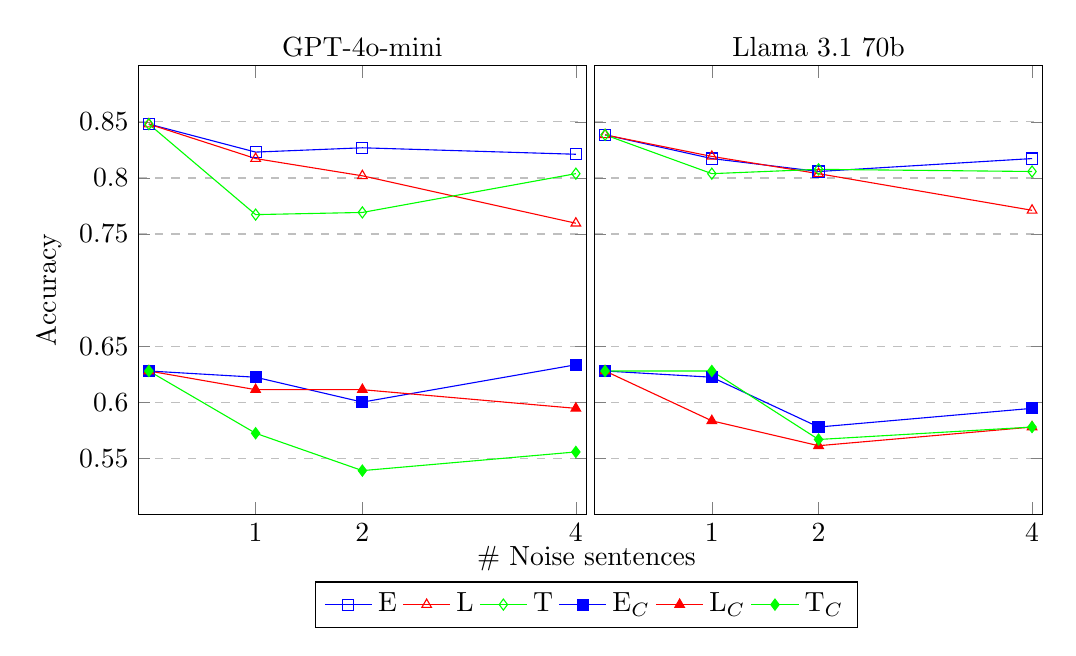
\begin{tikzpicture}
        \begin{axis}[name=gpt,
            title={GPT-4o-mini},
            width=0.6\linewidth,
            height=0.6\linewidth,
            xlabel={\# Noise sentences},
            ylabel={Accuracy},
            xmin=-0.1, xmax=4.1,
            ymin=0.5, ymax=0.9,
            xtick={1,2,4},
            ytick={0.55, 0.6, 0.65, 0.75, 0.8, 0.85},
            title style={yshift=-0.6em},
            legend style={at={(1,-0.15)},
	           anchor=north,legend columns=-1},
            x label style={at={(axis description cs:1,-0.05)},anchor=north},
            y label style={at={(axis description cs:-0.15,0.5)},anchor=south},
            ymajorgrids=true,
            grid style=dashed,
        ]
            \addplot[color=blue, mark=square,]
                coordinates {
                (0,0.848076939582825)(1,0.823076903820038)(2,0.826923072338104)(4,0.821153819561005)
                };
            \addplot[color=red, mark=triangle,]
                coordinates {
                (0,0.848076939582825)(1,0.817307710647583)(2,0.801923096179962)(4,0.759615361690521)
                };
            \addplot[color=green, mark=diamond,] 
                coordinates {
                (0,0.848076939582825)(1,0.767307698726654)(2,0.769230782985687)(4,0.803846180438995)
                };
            \addplot[color=blue, mark=square*] 
                coordinates {
                (0,0.627777755260468)(1,0.622222244739533)(2,0.600000023841858)(4,0.633333325386047)
                };
            \addplot[color=red, mark=triangle*,] 
                coordinates {
                (0,0.627777755260468)(1,0.611111104488373)(2,0.611111104488373)(4,0.594444453716278)
                };
            \addplot[color=green, mark=diamond*,] 
                coordinates {
                (0,0.627777755260468)(1,0.572222232818604)(2,0.538888871669769)(4,0.555555582046509)
                };
                \legend{E,L,T,$\text{E}_C$, $\text{L}_C$ , $\text{T}_C$}
        \end{axis}

        \begin{axis}[name=llama, at={($(gpt.east)+(0.1cm,0)$)},anchor=west,
            title={Llama 3.1 70b},
            width=0.6\linewidth,
            height=0.6\linewidth,
            xmin=-0.1,, xmax=4.1,
            ymin=0.5, ymax=0.9,
            xtick={1,2,4},
            ytick={0.55, 0.6, 0.65, 0.75, 0.8, 0.85},
            title style={yshift=-0.6em},
            yticklabel=\empty,
            ymajorgrids=true,
            grid style=dashed,
        ]
            \addplot[color=blue, mark=square,]
                coordinates {
                (0,0.838461518287659)(1,0.817307710647583)(2,0.805769205093384)(4,0.817307710647583)
                };
            \addplot[color=red, mark=triangle,]
                coordinates {
                (0,0.838461518287659)(1,0.819230794906616)(2,0.803846180438995)(4,0.771153867244721)
                };
            \addplot[color=green, mark=diamond,]
                coordinates {
                (0,0.838461518287659)(1,0.803846180438995)(2,0.807692289352417)(4,0.805769205093384)
                };
            \addplot[color=blue, mark=square*]
                coordinates {
                (0,0.627777755260468)(1,0.622222244739533)(2,0.577777802944183)(4,0.594444453716278)
                };
            \addplot[color=red, mark=triangle*,]
                coordinates {
                (0,0.627777755260468)(1,0.583333313465118)(2,0.561111092567444)(4,0.577777802944183)
                };
            \addplot[color=green, mark=diamond*,]
                coordinates {
                (0,0.627777755260468)(1,0.627777755260468)(2,0.566666662693024)(4,0.577777802944183)
                };
        \end{axis}
    \end{tikzpicture}
    \caption{Influence of the number of noisy sentences for FOL.}
    \label{fig:length_distraction}
\end{figure}



\subsection{Impact of Method Design}
\paragraph{\textbf{\emph{F4: \ac{CoT} prompting is most impactful when both noise and counterfactual perturbations are applied.}}}
The accuracies for the individual \acp{LLM} in Table~\ref{tab:distraction_k4_formalisation} show that the impact of \ac{CoT} is negligible for noise-only datasets (first four columns). Meanwhile, the benefit from \ac{CoT} is most pronounced in the datasets that combine noise and counterfactual perturbations.
The better-performing informal prompting strategy for a model remains stable for all types of distractions. Still, the decline in performance due to counterfactuals leads to a less consistent preference for a specific prompting style.

\paragraph{\textbf{\emph{F5: The best-performing grammar differs per model and is unstable across data versions.}}}

The evaluation of different logical forms for formal \ac{LLM}-based reasoning in Table~\ref{tab:distraction_k4_logical_form} shows the preference of some models for specific syntactic formats.
Llama 3.1 70B has a considerable improvement of $12\%$ with TPTP syntax on the original set, while Llama 3.1 8B benefits from the R-FOL syntax. However, all grammars show a declining accuracy trend and increased syntax errors for noise perturbations, where the best grammar loses its advantage over the rest. 
When comparing the grammars on the counterfactual partitions, we observe that TPTP is consistently more robust than the standard first-order logic grammar. Here, GPT 4o-mini shows a reduction from $O$ to $O_C$ of $20\%$ for FOL and only $12\%$ for the TPTP grammar. Since this does not correlate with fewer syntax errors, the formalisation in TPTP prevents semantical errors for counterfactual premises. 
A positive reading of these results, especially the minor differences between FOL and R-FOL, is that autoformalisation \acp{LLM} can adapt to the grammar syntax prescribed in the prompt without further loss in performance.

\begin{table}[!t]
\small
\setlength{\modelspacing}{2pt}
\setlength{\tabcolsep}{1.7pt} % Default value: 6pt
\setlength{\belowrulesep}{4pt}
\begin{threeparttable}
    \centering
    \begin{tabular}{cc l r rrr @{\quad} rrrr}
\toprule
\multirow{2}{*}{} & \multirow{2}{*}{} & Grammar & \multirow{2}{*}{O} & \multicolumn{3}{c}{Distraction} & \multicolumn{4}{c}{Counterfactual} \\
 & & Syntax & & E& L & T & $\text{O}_C$ & $\text{E}_C$& $\text{L}_C$ & $\text{T}_C$\\
\midrule
\multirow{6}{*}{\rotatebox{90}{Llama-3.1}} & \multirow{3}{*}{\rotatebox{90}{8B}} 
   & FOL & 0.77 & \textbf{0.71} & 0.61 & \textbf{0.53} & 0.58 & \textbf{0.55} & 0.52 & \textbf{0.56} \\
 & & R-FOL & \textbf{0.78} & 0.69 & \textbf{0.62} & \textbf{0.53} & 0.58 & \textbf{0.55} & \textbf{0.54} & 0.52 \\
 & & TPTP & 0.73 & 0.67 & 0.55 & 0.51 & \textbf{0.68} & 0.54 & 0.46 & 0.51 \\[\modelspacing]
\cmidrule{2-11}
 & \multirow{3}{*}{\rotatebox{90}{70B}} 
   & FOL & 0.76 & 0.73 & 0.71 & \textbf{0.72} & 0.67 & 0.57 & 0.63 & 0.56 \\
 & & R-FOL & 0.76 & 0.73 & 0.67 & 0.71 & 0.64 & 0.57 & 0.53 & 0.64 \\
 & & TPTP & \underline{\textbf{0.88}} & \underline{\textbf{0.84}} & \underline{\textbf{0.81}} & \textbf{0.72} & \underline{\textbf{0.81}} & \underline{\textbf{0.68}} & \underline{\textbf{0.67}} & \underline{\textbf{0.68}} \\[\modelspacing]
\midrule
\multirow{3}{*}{\rotatebox{90}{GPT}} & \multirow{3}{*}{\rotatebox{90}{4o-mini}} 
   & FOL & \textbf{0.84} & \textbf{0.82} & \textbf{0.72} & \underline{\textbf{0.78}} & 0.64 & \textbf{0.63} & \textbf{0.61} & 0.51 \\
 & & R-FOL & \textbf{0.84} & 0.77 & 0.70 & \underline{\textbf{0.78}} & \textbf{0.72} & 0.56 & 0.54 & \textbf{0.63} \\
 & & TPTP & 0.83 & \textbf{0.82} & 0.71 & 0.71 & 0.69 & \textbf{0.63} & 0.57 & 0.57 \\
\bottomrule
\end{tabular}
\caption{Accuracies of different formalisation grammars for autoformalisation.}
\label{tab:distraction_k4_logical_form}
\end{threeparttable}
\end{table} 

\paragraph{\textbf{\emph{F6: Feedback does not help \acp{LLM} self-correct to mitigate robustness issues.}}}
\autoref{tab:distraction_k4_feedback} shows the results with different error recovery mechanisms. The results indicate that no feedback strategy emerges as a winner in the different datasets. 
All feedback variants reduce syntax errors for noise perturbations, but given the lack of a consistent increase in accuracy, the corrected formalisations are most likely to contain semantic errors still. 
The type of feedback message only has a minor influence on correcting syntax errors, whereas Llama 3.1 70b and GPT 4o-mini correct slightly more syntax errors with specific error messages. This finding aligns with \cite{huang2023large}, who also found that \acp{LLM} cannot consistently self-correct their reasoning after receiving relevant feedback.

\begin{table}[!ht]
\small
\setlength{\modelspacing}{2pt}
\setlength{\tabcolsep}{1.7pt} % Default value: 6pt
\setlength{\belowrulesep}{4pt}
\begin{threeparttable}
    \centering
    \begin{tabular}{cc l r rrr @{\quad} rrrr}
\toprule
\multirow{2}{*}{} & \multirow{2}{*}{} & \multirow{2}{*}{Feedback} & \multirow{2}{*}{O} & \multicolumn{3}{c}{Distraction} & \multicolumn{4}{c}{Counterfactual} \\
 & & & & E& L & T & $\text{O}_C$ & $\text{E}_C$& $\text{L}_C$ & $\text{T}_C$\\
\midrule
\multirow{8}{*}{\rotatebox{90}{Llama-3.1}} & \multirow{4}{*}{\rotatebox{90}{8B}} 
   & No recovery & 0.77 & \textbf{0.72} & 0.62 & 0.53 & 0.59 & 0.58 & 0.56 & \textbf{0.56} \\
 & & Error type & \textbf{0.79} & 0.71 & 0.63 & \textbf{0.56} & \textbf{0.66} & 0.54 & 0.52 & 0.51 \\
 & & Error message & 0.78 & 0.71 & \textbf{0.67} & 0.55 & 0.59 & 0.53 & \underline{\textbf{0.64}} & 0.49 \\
 & & Warning & 0.74 & 0.66 & 0.58 & 0.55 & 0.55 & \textbf{0.60} & 0.49 & 0.49 \\[\modelspacing]
\cmidrule{2-11}
 & \multirow{4}{*}{\rotatebox{90}{70B}} 
   & No recovery & \textbf{0.77} & \textbf{0.72} & \textbf{0.73} & 0.71 & \textbf{0.64} & 0.59 & \textbf{0.61} & 0.56 \\
 & & Error type & 0.72 & 0.70 & 0.72 & \textbf{0.73} & 0.62 & 0.56 & 0.60 & 0.58 \\
 & & Error message & 0.71 & 0.70 & \textbf{0.73} & 0.71 & \textbf{0.64} & 0.59 & 0.54 & \underline{\textbf{0.64}} \\
 & & Warning & 0.69 & \textbf{0.72} & 0.72 & 0.72 & 0.62 & \underline{\textbf{0.65}} & \textbf{0.61} & 0.63 \\[\modelspacing]
\midrule
\multirow{4}{*}{\rotatebox{90}{GPT}} & \multirow{4}{*}{\rotatebox{90}{4o-mini}} 
   & No recovery & \underline{\textbf{0.84}} & \underline{\textbf{0.82}} & 0.73 & 0.79 & 0.64 & \textbf{0.62} & 0.56 & \textbf{0.56} \\
 & & Error type & 0.83 & 0.79 & 0.74 & 0.76 & 0.67 & 0.57 & 0.56 & \textbf{0.56} \\
 & & Error message & \underline{\textbf{0.84}} & 0.78 & \underline{\textbf{0.77}} & \underline{\textbf{0.80}} & 0.62 & 0.59 & 0.56 & \textbf{0.56} \\
 & & Warning & \underline{\textbf{0.84}} & 0.75 & 0.73 & 0.76 & \underline{\textbf{0.70}} & 0.61 & \textbf{0.61} & 0.55 \\
 \bottomrule
\end{tabular}
\caption{Accuracies of error recovery strategies.}
\label{tab:distraction_k4_feedback}
\end{threeparttable}
\end{table} 

\subsection{Error Analysis}
\label{subsec:errors}
\paragraph{\textbf{\emph{F7: Autoformalisation increases syntax errors for noise perturbations.}}}
The low performance for noise perturbations correlates with more syntax errors for all models and distraction categories (cf. execution rates in Table~\ref{tab:appendix_k4_formalisation_exec}). The three worst-performing models (both Mistral models, Gemma-2 9b) generate, at best, for $37\%$  and, at worst, for only $4\%$ of the samples, a valid logical form.
Gemma-2 9b and Llama3.1 8b produce more syntax errors than the larger counterparts, suggesting that larger models are more robust towards noise perturbations. 
The accuracy of syntactically valid samples is higher than the informal reasoning methods for most distractions (Table~\ref{tab:appendix_k4_formalisation_vacc}), motivating informal reasoning as a backup strategy for formal reasoning. The error message feedback reveals two common syntax errors: 1) errors by models with an initial low execution rate exhibit issues with the template structure, including using incorrect keywords or adding conversational phrases;
2) perturbation-related errors, the most common of which is using undefined truth constants as part of tautological distractions. 

\paragraph{\textbf{\emph{F8: Autoformalisation increases semantic errors for counterfactuals.}}}
Unlike the introduced noise, counterfactual perturbations do not lead to more syntax errors. The execution rate in Table~\ref{tab:appendix_k4_formalisation_exec} is stable or improves for counterfactuals. However, we see a drop in accuracy for the counterfactual column $\text{O}_C$ in Table~\ref{tab:distraction_k4_formalisation} and can conclude that the number of logical forms with semantic errors has to increase. This suggests that the introduced negation is not correctly formalised. Looking at the warnings generated by the feedback mechanism, for GPT 4o-mini, $161$ warning messages are generated on the unperturbed data. $54$ of these were fixed with a single iteration. Not considering predicates and individuals as part of the context is the most frequent warning across all models. 
\section*{Conclusion}
This paper aims to enhance our understanding of the computational complexity of computing various Shapley value variants. We found that for various ML models --- including decision trees, regression tree ensembles, weighted automata, and linear regression --- both local and global interventional and baseline SHAP can be computed in polynomial time under HMM modeled distributions. This extends popular algorithms, such as TreeSHAP, beyond their empirical distributional scope. We also establish strict complexity gaps between the various SHAP variants (baseline, interventional, and conditional) and prove the intractability of computing SHAP for tree ensembles and neural networks in simplified scenarios. Overall, we present SHAP as a versatile framework whose complexity depends on four key factors: \begin{inparaenum}[(i)] \item model type, \item SHAP variant, \item distribution modeling approach, \item and local vs. global explanations\end{inparaenum}. We believe this perspective provides deeper insight into the computational complexity of SHAP, paving the way for future work.




%We believe that our framework provides a more intricate understanding of SHAP computation complexity across different models, distributions, and variants, paving the way for further research.

Our work opens promising directions for future research. First, expanding our computational analysis to other SHAP-related metrics, such as asymmetric SHAP~\citep{frye20} and SAGE~\citep{covert2020understanding}, would be valuable. Additionally, we aim to explore more expressive distribution classes and relaxed assumptions beyond those in Section \ref{sec:tractable} while maintaining tractable SHAP computation. Finally, when exact computation is intractable (Section \ref{sec:intractable}), investigating the approximability of SHAP metrics through approximation and parameterized complexity theory~\citep{downey2012parameterized} is an important direction.

%Our work opens several promising avenues for future research on the computational properties of explainable AI methods, with a particular focus on SHAP. First, it would be interesting to broaden the computational analysis conducted in this work to include other popular SHAP-related metrics in the literature, such as asymmetric SHAP \cite{frye20} and SAGE \cite{covert2020understanding}. Also, in the future, we aim to explore more expressive distribution classes and relaxed distributional assumptions—extending beyond those examined in Section \ref{sec:tractable} —that still yield tractable SHAP computation. Finally, when exact computation proves intractable (Section \ref{sec:intractable}), it is worthwhile to theoretically investigate the question of the approximability of computing the SHAP metrics across various configurations, through the lens of approximation and parametrized complexity theory \cite{arora2009computational}.

%This paper aims to deepen our understanding of the computational complexity involved in obtaining different Shapley value variants. We found that for a variety of ML models, including decision trees, tree ensembles for regression, weighted automata, and linear regression models — computing both local and global interventional and baseline SHAP can be done in polynomial time when distributions are modeled by HMMs. This extends the distributional scope of popular algorithms like TreeSHAP, which is limited to empirical distributions. Additionally, we demonstrate a strict complexity gap between SHAP variants, showing that interventional and baseline SHAP can be strictly easier to compute than conditional SHAP. Despite these positive results, we uncovered intractability for various SHAP variants in neural networks and tree ensembles. Finally, we provided generalized complexity relations across SHAP variants. We believe that our framework offers a deeper understanding of the complexity involved in computing SHAP across various variants, models, distributions, as well as in both local and global computations, laying the groundwork for future research.
\section{Acknowledgement}
The authors are grateful to  Afonso S. Bandeira, Anastasia Kireeva, Alexander S. Wein, Samuel B. Hopkins, and Tim Kunisky for helpful discussions. 



% \bibliographystyle{IEEEtran}
% \footnotesize
% \bibliography{ref}

\footnotesize

\documentclass[conference, 9pt]{IEEEtran}

\usepackage[normalem]{ulem}
\usepackage{amsmath}
\usepackage{amsfonts}
\usepackage{hyperref}
\usepackage{graphicx}
\usepackage{cleveref}
\usepackage{amsthm}
\usepackage{algorithm, algpseudocode,subcaption}
\usepackage{xcolor}
\usepackage{tikz}
\usepackage{caption}
\usepackage{listings}
\usepackage{array}
\usepackage{booktabs}
\usepackage{diagbox}
\usepackage{float}
\usepackage{geometry}
\geometry{a4paper,margin=0.5in}
\newtheorem{condition}{Condition}
\newtheorem{claim}{Claim}
\newtheorem{example}{Example} 
\newtheorem{theorem}{Theorem}
\newtheorem{lemma}{Lemma} 
\newtheorem{proposition}{Proposition} 
\newtheorem{remark}{Remark}
\newtheorem{corollary}{Corollary}
\newtheorem{definition}{Definition}
\newtheorem{conjecture}{Conjecture}
\newtheorem{axiom}{Axiom}
\title{Robust Anomaly Detection via Tensor Pseudoskeleton Decomposition}
\author{Bowen Su }
\definecolor{officegreen}{rgb}{0.0, 0.5, 0.0}
\lstset{
    language=Python,
    basicstyle=\ttfamily\small,
    commentstyle=\color{blue},
    keywordstyle=\color{black},
    showstringspaces=false,
    numbers=left,
    numberstyle=\tiny,
    stepnumber=1,
    numbersep=5pt,
}



\begin{document}

\maketitle

\begin{abstract}
Anomaly detection plays a critical role in modern data-driven applications, from identifying fraudulent transactions and safeguarding network infrastructure to monitoring sensor systems for irregular patterns. Traditional approaches—such as distance-, density-, or cluster-based methods, face significant challenges when applied to high-dimensional tensor data, where complex interdependencies across dimensions amplify noise and computational complexity. To address these limitations, this paper leverages Tensor  pseudoskeleton decomposition within a tensor-robust principal component analysis framework to extract low-Tucker-rank structure while isolating sparse anomalies, ensuring robustness to anomaly detection. We establish theoretical analysis of convergence, and estimation error, demonstrating the stability and accuracy of the proposed approach. Numerical experiments on real-world spatiotemporal data from New York City taxi trip records validate the superiority of the proposed method in detecting anomalous urban events compared to existing benchmark methods. The results underscore the potential of Tensor  pseudoskeleton decomposition to enhance anomaly detection for large-scale, high-dimensional data.
\end{abstract}
\section{Introduction}
Anomaly detection is a crucial task in data analysis, with applications spanning various domains such as fraud detection~\cite{motie2024financial}, cybersecurity~\cite{wurzenberger2024analysis}, healthcare monitoring~\cite{kadir2024anomaly}, and sensor network analysis~\cite{tarish2025anomaly}. Anomalies, or outliers, represent data points or patterns that deviate significantly from the expected behavior, often signaling critical events or errors that require immediate attention. Detecting these anomalies, especially within high-dimensional and complex datasets, is challenging due to the sheer volume of data and the underlying noise that can mask unusual patterns.

Traditional anomaly detection techniques, including distance-based~\cite{Angiulli2002}, density-based~\cite{Breunig2000}, and clustering-based methods~\cite{Jiang2003,Hautamaki2004}, have shown some success in identifying anomalies in lower-dimensional datasets.
 However, these approaches often struggle when extended to high-dimensional tensor data, where intricate dependencies exist across multiple dimensions. Tensor data structures are common in fields such as video surveillance, biomedical imaging, and environmental monitoring, where data is naturally organized in multi-way arrays. The increased dimensionality not only complicates the detection of anomalies but also amplifies the computational costs, making scalability a critical concern.

In recent years, tensor decomposition methods have emerged as powerful tools for managing high-dimensional data. By transforming complex data into a lower-dimensional, interpretable form, tensor decompositions facilitate efficient storage, processing, and analysis. Among these methods, Tucker decomposition, a form of higher-order singular value decomposition, is particularly effective at capturing the core structure of tensor data. However, while Tucker decomposition enables significant dimensionality reduction, it remains sensitive to outliers, which can distort the decomposition and lead to unreliable results in anomaly detection.

To address these limitations,  Tensor  pseudoskeleton decomposition offers an alternative approach by selecting representative parts of the data, thereby preserving essential features while reducing redundancy.  Tucker pseudoskeleton decomposition provides a structured decomposition that is both computationally efficient and robust~\cite{hamm2023generalized,cai2021mode}. 

In this paper, we focus on anomaly detection within the tensor robust principal component analysis framework by leveraging a Tucker pseudoskeleton decomposition specifically tailored for high-dimensional datasets~\cite{hamm2023generalized,cai2021mode}. By incorporating sparsity and regularization constraints, our method reduces sensitivity to anomalies, enabling more accurate and resilient detection of unusual patterns. The Tucker  pseudoskeleton decomposition framework combines the strengths of Tucker decomposition’s structural insight with pseudoskeleton’s selective feature extraction while enhancing robustness against outliers~\cite{hamm2023generalized}.


\subsection{Notations and definitions}
In this section, we introduce notation and review foundational properties of Tucker-based tensor decomposition, which will be essential throughout the chapter. Tucker decomposition serves as a powerful tool for capturing the core structure of high-dimensional data, providing both a compact representation and interpretability of multi-dimensional relationships within the data.

To distinguish between different mathematical entities, we adopt the following conventions: calligraphic capital letters (e.g., $\mathcal{T}$) represent tensors, regular uppercase letters (e.g., ${X}$) denote matrices, regular lowercase letters (e.g., ${x}$) indicate vectors or scalars. For submatrices, $[X]_{I,:}$ and $[X]_{:,J}$ refer to the rows and columns of matrix ${X}$ indexed by sets $I$ and $J$, respectively. For tensors, $[\mathcal{T}]_{I_1, \dots, I_n}$ represents a subtensor of $\mathcal{T}$ with index sets $I_k$ along each mode $k$. A specific element in a tensor is accessed by the index notation $[\mathcal{T}]_{i_1, \dots, i_n}$. 

The tensor norm used in this chapter is the Frobenius norm~\cite{kolda2009tensor}, defined for a tensor \(\mathcal{T}\) as:
\begin{equation*}
    \|\mathcal{T}\|_\mathrm{F} = \sqrt{\sum_{i_1, \dots, i_n} [\mathcal{T}]_{i_1, \dots, i_n}^2}.
\end{equation*}
This norm represents the square root of the sum of the squared entries of \(\mathcal{T}\), extending the Frobenius norm from matrices to higher-order tensors.
For matrices, the Moore-Penrose Pseudoinverse is denoted by ${X}^\dagger$. The notation $[d] := \{1, \dots, d\}$ represents the set of natural numbers up to $d$.

\begin{definition}[\textbf{Tensor Matricization/Unfolding}~\cite{kolda2009tensor}]
    An $n$-mode tensor $\mathcal{T}$ can be reshaped into a matrix by unfolding it along each of its $n$ modes. The mode-$k$ unfolding of a tensor $\mathcal{T} \in \mathbb{R}^{d_1 \times \dots \times d_n}$, denoted $\mathcal{T}_{(k)}$, is a matrix of size $\mathbb{R}^{d_k \times \prod_{j \neq k} d_j}$, obtained by arranging all vectors of $\mathcal{T}$ with indices fixed in all modes except the $k$-th. This transformation, $\mathcal{T} \mapsto \mathcal{T}_{(k)}$, is referred to as the mode-$k$ unfolding operator.
\end{definition}

\begin{definition}[\textbf{Mode-$k$ Product}~\cite{kolda2009tensor}]
    Let $\mathcal{T} \in \mathbb{R}^{d_1 \times \dots \times d_n}$ and ${A} \in \mathbb{R}^{J \times d_k}$. The mode-$k$ product of $\mathcal{T}$ with ${A}$, denoted by $\mathcal{Y} = \mathcal{T} \times_k {A}$, is defined element-wise as:
    \begin{equation*}
        [\mathcal{Y}]_{i_1, \dots, i_{k-1}, j, i_{k+1}, \dots, i_n} = \sum_{s=1}^{d_k} [\mathcal{T}]_{i_1, \dots, i_{k-1}, s, i_{k+1}, \dots, i_n} [{A}]_{j, s}.
    \end{equation*}
    Alternatively, this operation can be represented in matrix form as $\mathcal{Y}_{(k)} = {A} \mathcal{T}_{(k)}$. For a sequence of tensor-matrix products across different modes, we use the notation $\mathcal{T} \times_{i=t}^{s} {A}_i$ to indicate the product $\mathcal{T} \times_{t} {A}_{t} \times_{t+1} \dots \times_{s} {A}_{s}$. This operation is referred to as the `tensor-matrix product' throughout the paper.
\end{definition}
\begin{definition}[\textbf{Tucker Rank and Tucker Decomposition}~\cite{kolda2009tensor}]
    The Tucker decomposition of a tensor $\mathcal{T}$ approximates it by expressing it as a product of a core tensor $\mathcal{C}$ and factor matrices ${A}_k$ along each mode:
    \begin{equation*}\label{eqn:Tucker_Decomposition}
        \mathcal{T} \approx \mathcal{C} \times_{i=1}^n {A}_i.
    \end{equation*}
    If the approximation in \eqref{eqn:Tucker_Decomposition} becomes an equality and the core tensor $\mathcal{C} \in \mathbb{R}^{r_1 \times \dots \times r_n}$, this is termed an exact Tucker decomposition of $\mathcal{T}$. The ranks $(r_1, \dots, r_n)$ are known as the Tucker ranks of the tensor $\mathcal{T}$.
\end{definition}

%\begin{remark}
%    Tucker decomposition can be viewed as a generalization of matrix singular value decomposition (SVD) to higher dimensions, preserving essential structure while reducing dimensionality. The HOSVD~\cite{de2000best} is a specific orthogonal form of Tucker decomposition commonly used in applications.
%\end{remark}
In the realm of matrix algebra, the pseudoskeleton decomposition technique is a good alternative to SVD~\cite{Goreinov}. Specifically, this method entails selecting specific columns ${C}$ and rows ${R}$ from a matrix ${X} \in \mathbb{R}^{d_1 \times d_2}$, and constructing a core matrix ${U} = {X}(I, J)$. The matrix ${X}$ is then reconstructed through the product ${C} {U}^\dagger {R}$, under the condition that $\operatorname{rank}({U}) = \operatorname{rank}({X})$. Expanding from matrices to tensors, the initial adaptations of pseudoskeleton decompositions applied a single-mode unfolding to 3-mode tensors~\cite{mahoney2008tensor}. To my best knowledge, the following are recent works on tensor pseudoskeleton decompositions or Tensor CUR Decompostions~\cite{hamm2023generalized,cai2021mode,cai2023robust,ahmadi2022cross,caiafa2010generalizing}. Furthermore, H. Cai, K. Hamm, and etc have presented rigorous theoretical results on the exact tensor pseudoskeleton decomposition \cite{cai2021mode,cai2023robust,hamm2023generalized}. For completeness, we present their work below.
\begin{definition}[Tensor pseudoskeleton decompositions or Tensor CUR Decompostions~\cite{hamm2023generalized,cai2021mode,cai2023robust}]
 Consider a tensor \(\mathcal{A} \in \mathbb{R}^{d_1 \times \cdots \times d_n}\) with Tucker ranks \((r_1, \dots, r_n)\). Suppose that for each mode \(i\), there exists a subset \(I_i \subseteq [d_i]\) such that 
 \[
\mathcal{A} = \mathcal{R} \times_{i=1}^{n} \left( C_i U_i^\dagger \right),
\]
where \(\mathcal{R} = [\mathcal{A}]_{I_1, \dots, I_n}, \quad C_i = [\mathcal{A}_{(i)}]_{:, J_i}, \quad \text{and} \quad U_i = [\mathcal{C}_{(i)}]_{I_i, :}, \quad J_i = \bigotimes_{j \neq i} I_j.
\)
\end{definition}
\begin{theorem}[{~\cite{hamm2023generalized,cai2021mode,cai2023robust}}]\label{thm:  Tucker Decomposition}
    For a tensor $\mathcal{A} \in \mathbb{R}^{d_1 \times \cdots \times d_n}$ with Tucker ranks $(r_1, \dots, r_n)$, consider subsets $I_i \subseteq [d_i]$ and let $J_i = \bigotimes_{j \neq i} I_j$ for each mode $i$. Define $\mathcal{R} = [\mathcal{A}]_{I_1, \dots, I_n}$, ${C}_i = [\mathcal{A}_{(i)}]_{:, J_i}$, and ${U}_i = [\mathcal{C}_{(i)}]_{I_i, :}$. The following conditions are equivalent:
    \begin{enumerate}
        \item $\mathcal{A} = \mathcal{R} \times_{i=1}^{n} ({C}_{i} {U}_i^\dagger)$,
        \item $\operatorname{rank}({U}_i) = r_i$ for all $i$,
        \item $\operatorname{rank}({C}_i) = r_i$ for all $i$, and $\mathcal{R}$ has Tucker rank $(r_1, \dots, r_n)$.
    \end{enumerate}
\end{theorem}
 For those interested in further details, It is recommended to read works~\cite{hamm2023generalized,cai2021mode,ahmadi2022cross,caiafa2010generalizing,cai2023robust,che2022perturbations,saibaba2016hoid}.



\section{Methodology}
We employ Tensor Robust Principal Component Analysis, an extension of classical Robust PCA that can operate directly on multi-dimensional (tensor) data. Unlike conventional low-rank models that assume the entire dataset is low-rank, TRPCA decomposes a given tensor into two distinct components: a low-rank component representing regular patterns and a sparse component isolating anomalies. This decomposition effectively isolates outliers in spatial-temporal data while retaining core structural patterns, providing a more flexible and robust approach to anomaly detection. By handling high-dimensional tensor data, TRPCA is particularly well-suited for scenarios where data is naturally structured as a multi-way array, allowing for the detection of unusual patterns that vary across both space and time.

In this framework, we represent the spatial-temporal data as a tensor $\mathcal{T} \in \mathbb{R}^{d_1 \times d_2 \times \cdots \times d_n}$, where each dimension $d_i$ corresponds to a specific mode of the data. For example, $d_1$ might represent spatial coordinates, $d_2$ temporal intervals, and additional dimensions might capture contextual features or sensor types. The objective is to decompose $\mathcal{T}$ into two components: a low-rank tensor $\mathcal{L}^\star$ that captures the dominant spatial-temporal structure, and a sparse tensor $\mathcal{S}^\star$ representing anomalies or outliers. The decomposition is expressed as:
\begin{equation*}
    \mathcal{T} = \mathcal{L}^\star + \mathcal{S}^\star,
\end{equation*}
where $\mathcal{L}^\star \in \mathbb{R}^{d_1 \times \cdots \times d_n}$ encapsulates the smooth, regular patterns in the data, while $\mathcal{S}^\star \in \mathbb{R}^{d_1 \times \cdots \times d_n}$ captures deviations from these patterns, isolating events that significantly differ from expected behavior. This separation allows for robust anomaly detection, as $\mathcal{S}^\star$ can pinpoint localized irregularities without interference from the regular structure. Mathematically, we formulate the anomaly detection problem as an optimization problem that seeks to minimize the reconstruction error between $\mathcal{T}$ and the sum of $\mathcal{L}$ and $\mathcal{S}$. This is achieved through the following objective:
\begin{equation*}\label{eq:trpca_formulation}
    \begin{split}
        \min_{\mathcal{R}, {C}_{i}, {U}_i, \mathcal{S}} & \quad \|\mathcal{T} - \mathcal{L} - \mathcal{S}\|_\mathrm{F} \\
        \text{subject to} & \quad \mathcal{L}= { \mathcal{R} \times_{i=1}^{n} ({C}_{i} {U}_i^\dagger)}\\
        &\quad\|\mathcal{S}\|_{\infty} \leq \alpha.
    \end{split}
\end{equation*}






\subsection{TRPCA via Tensor 
Pseudoskeleton Decomposition}

\begin{algorithm}[H]
    \caption{TRPCA via Tensor 
Pseudoskeleton Decomposition}
    \label{alg:TCPD}
    \begin{algorithmic}[1]
        \State \textbf{Input: } $\mathcal{T}  \in \mathbb{R}^{d_1 \times \cdots \times d_n}$: observed tensor; 
        $(r_1, \cdots, r_n)$: estimated Tucker rank; 
        $\varepsilon$: targeted precision; 
        $\zeta^{(0)}, \gamma$: thresholding parameters; $\{|I_i|\}_{i=1}^n,\{|J_i|\}_{i=1}^n$: cardinalities for sample indices.
        \State  Uniformly sample the indices $\{I_i\}_{i=1}^n, \{J_i\}_{i=1}^n$ 
        \State \textbf{Initialization:} $\mathcal{L}^{(0)} = 0, \mathcal{S}^{(0)} = 0, k = 0$
        \While {$e^{(k)} > \varepsilon$}
            \State \textcolor{officegreen}{// Step (I): Updating $\mathcal{S}$}
            \State $\zeta^{(k+1)} = \gamma \cdot \zeta^{(k)}$ 
            \State $\mathcal{S}^{(k+1)} = \mathrm{HT}_{\zeta^{(k+1)}}(\mathcal{T} - \mathcal{L}^{(k)})$  
            \State \textcolor{officegreen}{// Step (II): Updating $\mathcal{L}$}
            \State $\mathcal{L}^{(k+1)} = [\mathcal{T} - \mathcal{S}^{(k+1)}]_{I_1, \cdots, I_n}$
            \For{$i = 1, \cdots, n$}
                \State $C_i^{(k+1)} = [(\mathcal{T} - \mathcal{S}^{(k+1)})_{(i)}]_{:, J_i}$ 
                %\State $U_i^{(k+1)} = \mathcal{H}_{r_i}([C_i^{(k+1)}]_{I_i, :})$ 
                \State $[Q,R] = \operatorname{qr}\left([C_i^{(k+1)}]_{I_i, :}^{\top}\right)$

             \State$\mathcal{L}^{(k+1)} = \mathcal{L}^{(k+1)} \times C_i^{(k+1)}[Q]_{:,:r}[R]_{:r,:}^{\dagger}$    
            \EndFor
            
            \State $k = k + 1$ 
        \EndWhile
        \State \textbf{Output: } $\mathcal{L}^{(k+1)}, \mathcal{S}^{(k+1)}$.
    \end{algorithmic}
\end{algorithm}

\subsubsection{Step~(I): Update Sparse Component $\mathcal{S}$} 
\label{sec:updateS}
In this step, we update the sparse component \(\mathcal{S}\) — which captures data outliers — using the technique described in \cite{cai2023robust,netrapalli2014non,cai2019accelerated}. Specifically, we apply an iterative decaying threshold within the hard thresholding operator \(\mathrm{HT}_\zeta\) paired with \(\gamma\), as described in \cite{cai2023robust,CaiR2024}.
The hard thresholding operator $\mathrm{HT}_\zeta$ is defined as follows:

\begin{equation*}
    [\mathrm{HT}_{\zeta}(\mathcal{T})]_{i_1,\cdots,i_n} =
    \begin{cases}
        [\mathcal{T}]_{i_1,\cdots,i_n}, & \quad |[\mathcal{T}]_{i_1,\cdots,i_n}| > \zeta; \\
        0,  & \quad \text{otherwise.}
    \end{cases}
\end{equation*}

This operator $\mathrm{HT}_\zeta$ effectively filters out entries with magnitudes less than or equal to $\zeta$, treating them as negligible. By applying this to the tensor $\mathcal{T}$, only values deemed significant (i.e., values exceeding the threshold) remain in the updated sparse component $\mathcal{S}$, thereby enhancing the sparsity of $\mathcal{S}$.
\subsubsection{Step~(II): Update Low-Tucker-rank Component $\mathcal{L}$}
\label{sec:updateL}
In this step, we aim to update the low-Tucker-rank component \(\mathcal{L}\), which models the structured, low-rank part of the data tensor via tensor pseudoskeleton decomposition. The update process is divided into two key stages: subspace identification and projective reconstruction.
To approximate the low-rank structure along each mode, we begin by extracting the mode-\(i\) fibers from the residual tensor \(\mathcal{T} - \mathcal{S}^{(k)}\), which represents the current estimate of the sparse component subtracted from the observed data tensor. The fibers are assembled into the matrix representation:
\[
C_i^{(k)} \in \mathbb{R}^{d_i \times |J_i|},
\]
where each column of \(C_i^{(k)}\) corresponds to a mode-\(i\) fiber indexed by a subset of indices \(J_i\). We select a subset of mode-\(i\) fibers indexed by \(I_i \subseteq \{1, \dots, d_i\}\) and perform an economy-size QR decomposition on the transposed submatrix formed by these selected fibers:
\begin{equation*}
    \left[C_i^{(k)}\right]_{I_i,:}^\top = Q R,
\end{equation*}
where \(Q \in \mathbb{R}^{|J_i| \times r_i}\) is a matrix with orthonormal columns representing the estimated basis, and \(R \in \mathbb{R}^{r_i \times |I_i|}\) is an upper triangular matrix. The dimension \(r_i\) is the estimated Tucker rank along mode-\(i\). This step yields a low-dimensional orthonormal basis that approximates the column space of the matricized low-rank component along mode-\(i\), i.e., the dominant subspace of \(\mathcal{L}^\star_{(i)}\).
Once the subspace is identified, we project the full set of mode-\(i\) fibers onto this estimated low-rank subspace. This is achieved by updating the mode-\(i\) factor matrix of the Tucker decomposition as follows:
\begin{equation*}
    \mathcal{L}^{(k+1)} \leftarrow \mathcal{L}^{(k+1)} \times_i \left( C_i^{(k)} \left[Q\right]_{:,:r_i} \left[R\right]_{:r_i,:}^\dagger \right).
\end{equation*}
This projection aligns the updated factor matrices along mode-\(i\) with the estimated low-dimensional subspace. Using QR decomposition and projecting onto the selected subspace, the computational complexity for each mode is reduced from the cubic cost \(\mathcal{O}(d_i^3)\) to the more efficient:
\(
\mathcal{O}(d_i r_i^2 + r_i^3),
\)
where \(d_i\) is the dimension along mode-\(i\), and \(r_i\) is the target Tucker rank. This reduction is particularly beneficial when the Tucker rank \(r_i\) is significantly smaller than the mode dimension \(d_i.\)



\section{Theoretical Foundations}\label{sec:theory}

\begin{theorem}\label{thm:subspace}
Let $\mathcal{L}^\star \in \mathbb{R}^{d_1 \times \cdots \times d_n}$ be a rank-$(r_1,\ldots,r_n)$ Tucker tensor with factor matrices $\mathbf{U}_i \in \mathbb{R}^{d_i \times r_i}$ satisfying the $\mu$-incoherence condition:
\begin{equation*}
\max_{1 \leq j \leq d_i} \|\mathbf{U}_i(j,:)\|_2 \leq \sqrt{\frac{\mu r_i}{d_i}}, \quad \forall i \in [n].
\end{equation*}
For any mode $i$ and failure probability $\delta \in (0,1)$, if we sample row indices $I_i \subseteq [d_i]$ with cardinality 
\begin{equation*}
|I_i| \geq c_0 \mu r_i \log^3\left(\frac{\mu r_i}{\delta}\right),
\end{equation*}
then with probability at least $1-\delta$, the sampled factor matrix satisfies
\begin{equation*}
\frac{1}{2}\sqrt{\frac{|I_i|}{d_i}} \leq \sigma_{\min}\left(\mathbf{U}_i(I_i,:)\right) \leq \sigma_{\max}\left(\mathbf{U}_i(I_i,:)\right) \leq \frac{3}{2}\sqrt{\frac{|I_i|}{d_i}},
\end{equation*}
where $c_0 > 0$ is an absolute constant and $\sigma_{\min}(\cdot)$, $\sigma_{\max}(\cdot)$ denote extremal singular values.
\end{theorem}
\begin{proof}
Define the normalized sampling matrix $\mathbf{\Phi}_i = \sqrt{\frac{d_i}{|I_i|}}\mathbf{S}_i$ where $\mathbf{S}_i \in \{0,1\}^{|I_i|\times d_i}$ has exactly one 1 per row. The subsampled matrix becomes:
\[
\widetilde{\mathbf{U}}_i = \mathbf{\Phi}_i\mathbf{U}_i \in \mathbb{R}^{|I_i|\times r_i}.
\]
Applying the matrix Bernstein inequality \cite{tropp2015introduction} to $\mathbf{U}_i\mathbf{U}_i^\top$:
\[
\mathbb{P}\left(\left\|\widetilde{\mathbf{U}}_i\widetilde{\mathbf{U}}_i^\top - \mathbf{I}\right\|_2 \geq t\right) \leq 2r_i \exp\left(-\frac{t^2|I_i|}{C\mu r_i \log d_i}\right).
\]

Setting $t = 1/2$ and solving for $|I_i|$:
\[
|I_i| \geq C\mu r_i \log^3\left(\frac{\mu r_i}{\delta}\right) \implies \frac{1}{2}\mathbf{I} \preceq \widetilde{\mathbf{U}}_i\widetilde{\mathbf{U}}_i^\top \preceq \frac{3}{2}\mathbf{I}.
\]

Notice that
\[
\sigma_{\min}^2(\mathbf{U}_i(I_i,:)) = \frac{d_i}{|I_i|}\sigma_{\min}^2(\widetilde{\mathbf{U}}_i) \geq \frac{d_i}{2|I_i|}.
\]
Similarly for $\sigma_{\max}$. Rearrangement completes the proof.
\end{proof}
\begin{theorem}\label{thm:convergence}
Under the conditions of Theorem \ref{thm:subspace} and assuming $\|\mathcal{S}^\star\|_\infty \leq \frac{\zeta^{(0)}}{2\sqrt{\log d_{\max}}}$, the iterates satisfy:
\begin{equation*}
\|\mathcal{L}^{(k+1)} - \mathcal{L}^\star\|_F \leq \rho\|\mathcal{L}^{(k)} - \mathcal{L}^\star\|_F + C\sqrt{\frac{\log d_{\max}}{|I|}}\|\mathcal{S}^\star\|_\infty,
\end{equation*}
where the contraction factor \[\rho = \max_{1 \leq i \leq n} \left(1 - \frac{\sigma_{\min}^2(\mathbf{U}_i(I_i,:))}{2}\right) < 1\] and $|I| = \min\limits_i |I_i|$.
\end{theorem}

\begin{proof}
Define the errors:
\[
\Delta^{(k)} := \mathcal{L}^{(k)} - \mathcal{L}^\star, \quad \mathcal{E}^{(k)} := \mathcal{S}^{(k)} - \mathcal{S}^\star
\]
The update rule induces coupled dynamics:
\[
\Delta^{(k+1)} = \underbrace{\sum_{i=1}^n (\mathcal{P}_{\mathbf{Q}_i^{(k)}} - \mathcal{P}_{\mathbf{U}_i})\Delta^{(k)}}_{\text{Projection error}} + \underbrace{\mathcal{B}^{(k)}\mathcal{E}^{(k)}}_{\text{Sparsity propagation}}
\]
where $\mathcal{B}^{(k)}$ represents the multi-modal projection of residual errors.
From the hard thresholding operation and incoherence condition:
\begin{align}
\|\mathcal{E}^{(k)}\|_1 &\leq \gamma\|\mathcal{E}^{(k-1)}\|_1 + C_1\|\Delta^{(k)}\|_F \\
&\leq \gamma^k\|\mathcal{E}^{(0)}\|_1 + C_1\sum_{m=0}^{k-1}\gamma^{k-m-1}\|\Delta^{(m)}\|_F
\end{align}
Under the sparsity condition $\|\mathcal{S}^\star\|_\infty \leq \frac{\zeta^{(0)}}{2\sqrt{\log d_{\max}}}$:
\[
\|\mathcal{B}^{(k)}\mathcal{E}^{(k)}\|_F \leq C_2\sqrt{\log d_{\max}}\|\mathcal{S}^\star\|_\infty
\]
Using Wedin's theorem \cite{wedin1972perturbation} and Theorem \ref{thm:subspace}:
\[
\|\mathcal{P}_{\mathbf{Q}_i^{(k)}} - \mathcal{P}_{\mathbf{U}_i}\|_2 \leq C_3\sqrt{\frac{\mu r_i d_i \log d_i}{|I_i|^2}}
\]
Summing over all modes:
\[
\left\|\sum_{i=1}^n (\mathcal{P}_{\mathbf{Q}_i^{(k)}} - \mathcal{P}_{\mathbf{U}_i})\Delta^{(k)}\right\|_F \leq \left(1 - \frac{c}{|I|}\right)\|\Delta^{(k)}\|_F
\]
Combining both components:
\begin{align}
\|\Delta^{(k+1)}\|_F &\leq \left(1 - \frac{c}{|I|}\right)\|\Delta^{(k)}\|_F + C_2\sqrt{\log d_{\max}}\|\mathcal{S}^\star\|_\infty \\
&\leq \rho\|\Delta^{(k)}\|_F + C\sqrt{\frac{\log d_{\max}}{|I|}}\|\mathcal{S}^\star\|_\infty
\end{align}
where $\rho = 1 - \frac{c}{2|I|}$. Solving the recursion completes the proof.
\end{proof}

\begin{lemma}\label{lem:Sparsity}
The projected sparsity term satisfies:
\[
\|\mathcal{B}^{(k)}\mathcal{E}^{(k)}\|_F \leq C\sqrt{\frac{\log d_{\max}}{|I|}}\left(\|\mathcal{E}^{(k)}\|_1 + \|\Delta^{(k)}\|_F\right)
\]
\end{lemma}

\begin{proof}
Decompose the sparsity propagation using the following inequality:
\[
\|\mathcal{B}^{(k)}\mathcal{E}^{(k)}\|_F \leq \|\mathcal{B}^{(k)}\|_F\|\mathcal{E}^{(k)}\|_1
\]
From Theorem \ref{thm:subspace}, the projection operator norm is bounded by:
\[
\|\mathcal{B}^{(k)}\|_F \leq C\sqrt{\frac{\log d_{\max}}{|I|}}
\]
Combining with the threshold error bound completes the proof.
\end{proof}
\begin{theorem}\label{thm:error}
After $K = \mathcal{O}\left(\frac{\log(1/\epsilon)}{\log(1/\rho)}\right)$ iterations, the estimation error decomposes as:
\begin{equation*}
\|\mathcal{L}^{(K)} - \mathcal{L}^\star\|_F \leq \underbrace{C_1\sqrt{\frac{r_{\max}d_{\max}\log d_{\max}}{|I|}}}_{\text{Approximation Error}} + \underbrace{C_2\frac{\|\mathcal{S}^\star\|_\infty}{\sqrt{\log d_{\max}}}}_{\text{Optimization Error}},
\end{equation*}
where $r_{\max} = \max_i r_i$, $d_{\max} = \max_i d_i$, and $C_1, C_2 > 0$ are constants.
\end{theorem}

\begin{proof}
From Theorem \ref{thm:subspace}:
\[
\|\mathcal{L}^{(0)} - \mathcal{L}^\star\|_F \leq C\sqrt{\frac{r_{\max}d_{\max}}{|I|}}.
\]
Applying Theorem \ref{thm:convergence} recursively:
\[
\|\mathcal{L}^{(K)} - \mathcal{L}^\star\|_F \leq \rho^K C\sqrt{\frac{r_{\max}d_{\max}}{|I|}} + \frac{C'\sqrt{\log d_{\max}}}{1-\rho}\|\mathcal{S}^\star\|_\infty.
\]
Setting $\rho^K \leq \sqrt{\frac{\log d_{\max}}{r_{\max}d_{\max}}}$ yields the optimal error decomposition.
\end{proof}

\begin{corollary}[Sample Complexity]\label{cor:sample}
To achieve $\epsilon$-accuracy with $\epsilon < \|\mathcal{S}^\star\|_\infty/\sqrt{\log d_{\max}}$, the required sampling complexity per mode is:
\begin{equation*}
|I_i| \geq C\mu r_i d_i \log^3 d_i \left(\frac{r_{\max}d_{\max}}{\epsilon^2} + \frac{\|\mathcal{S}^\star\|_\infty^2}{\epsilon^2\log d_{\max}}\right).
\end{equation*}
\end{corollary}




\section{Numerical Experiments}
We utilize the NYC yellow taxi trip records from 2018 as a real-world spatiotemporal dataset~\cite{indibi2024spatiotemporal,sofuoglu2022gloss}. This dataset provides a detailed log of each taxi trip, including departure and arrival information (zones and times), the number of passengers, and tip amounts. 

In our experiments, we aggregate the data same as that in ~\cite{indibi2024spatiotemporal} by counting the number of arrivals per zone over hourly intervals. To ensure statistical significance, we restrict our analysis to 81 central zones, which represent high-traffic areas and exclude zones with minimal activity. This selection reduces noise from sparsely populated zones and provides a more robust representation of NYC’s high-demand regions.
With these parameters, we constructed a four-dimensional tensor \( \mathbf{Y} \) with dimensions \( 24 \times 7 \times 53 \times 81 \). The modes of this tensor are defined as follows: the first mode corresponds to the 24 hours of a day; the second mode represents the 7 days of the week; the third mode encompasses the 53 weeks of the year; the fourth mode covers the 81 selected central zones in New York City. Thus, each entry  in the tensor represents the count of taxi arrivals for hour \( h \), day \( d \), week \( w \), and zone \( z \), aggregate over the year. 

We evaluate our anomaly detection approach by identifying the top \(K\%\) of entries with the highest anomaly scores from the extracted sparse tensors, with \(K\) varying across multiple thresholds (0.014, 0.07, 0.14, 0.3, 0.7, 1, 2, and 3). Each top-\(K\%\) subset is then compared to compiled event list to determine how many events are correctly detected. The compiled event list is chosen same as~\cite{sofuoglu2022gloss,indibi2024spatiotemporal}.\Cref{tab:events} compares the number of events detected by our method against five benchmark methods—LR-STSS~\cite{indibi2024spatiotemporal}, LR-TS~\cite{indibi2024spatiotemporal}, LR-SS~\cite{indibi2024spatiotemporal}, and HoRPCA~\cite{li2015low, geng2014high}—across different \(K\%\) thresholds.
 The parameters for our method are set as follows: a maximum of 150 iterations, a tolerance level of \(10^{-7}\), and a Tucker rank of \((26, 6, 4, 10)\). The parameters for the other four methods are adopted from \cite{indibi2024spatiotemporal}. %The RCURC algorithm was developed specifically for a specialized random sampling framework known as the Cross Concentrated Sampling model~\cite{cai2024robust}. Thus, to apply the RCURC algorithm, we first flatten the tensor along its spatial dimension, transforming it into a matrix of size \(81 \times 8904\). Next, we perform robust CCS sampling, where rows and columns are selected based on a uniform observation rate across submatrices and a specified percentage of sampled indices. Finally, the RCURC algorithm is applied to extract the low-rank structure of the flatten matrix. The parameter settings for RCURC are as follows: the maximum number of iterations is fixed at 200, sampling densities (\(\delta\)) range from 0.1 to 0.8, tolerance levels (\(\text{tol}\)) are set to \(1 \times 10^{-5}\), outlier amplification factors (\(c\)) vary from 0.0 to 0.4, and the rank parameter \(r\) is incremented sequentially from 1 to 40. Parameters of all other four methods are same as in~\cite{indibi2024spatiotemporal}.


\begin{table}[H]
\centering
\resizebox{0.5\textwidth}{!}{%
\begin{tabular}{|c|c|c|c|c|c|c|c|c|}
\hline
\%       & 0.014 & 0.07 & 0.14 & 0.3  & 0.7  & 1    & 2    & 3    \\ \hline
Ours    & \textbf{3}     & \textbf{6} & \textbf{10} & \textbf{14} & \textbf{16} & \textbf{18} & \textbf{20} & \textbf{20} \\ \hline
LR-STSS  & \textbf{3} & {4} & {7} & {12} & {15} & {17} & {19} & {19} \\ \hline
LR-TS    & 3     & 4     & 5     & 6     & 13    & 13    & 18    & 19    \\ \hline
LR-SS    & 1     & 1     & 2     & 3     & 5     & 6     & 13    & 16    \\ \hline
%RCURC    & 0     & 0     & 1     & 1     & 5     & 8     & {11}  & {12}  \\ \hline
HoRPCA   & 0     & 0     & 2     & 2     & 2     & 3     & 7     & 10    \\ \hline
\end{tabular}%
}
\caption{Number of detected events among 20 compiled events in NYC for varying top-\(K\%\) of the anomaly scores}
\label{tab:events}
\end{table}
\begin{figure}
    \centering
    \includegraphics[width=1\linewidth]{methods_runtime.png}
    \caption{Running Time}
    \label{fig:time}
\end{figure}
As shown in Table~\ref{tab:events} and \Cref{fig:time}, \Cref{alg:TCPD} not only achieves higher event detection accuracy across various thresholds but also significantly reduces running time compared to LR-STSS, LR-TS, LR-SS, and HoRPCA. This balance of efficiency and effectiveness underscores \Cref{alg:TCPD}’s practical advantages for large-scale or real-time anomaly detection scenarios. This performance affirms the efficacy of our model parameters, including a Tucker rank configuration suited for complex, multi-dimensional datasets.
\section{Conclusion}

In this short paper, we investigate the application of tensor  pseudoskeleton decomposition for anomaly detection in high-traffic areas of New York City. Specifically, we aim to capture temporal and spatial patterns in taxi arrival data. By focusing on central zones with significant activity, the result demonstrates its possibility of  tensor  pseudoskeleton decomposition to remove sparsity and highlight urban regions with high demand. 

\bibliographystyle{IEEEtran}
\bibliography{reference}
\end{document}

\end{document}
